%-------------------------------------------------------------------------
% INFORMACIÓN DEL ARTÍCULO
\thispagestyle{portadapage}
\setcounter{subsection}{0}
\setcounter{subsubsection}{0}
\setcounter{actividad}{0}
\setcounter{actividad_previa}{0}
\setcounter{actividad_entre}{0}
\renewcommand{\articulotipo}{Comunicación breve}
\renewcommand{\articulotitulo}{Redefiniendo el sentido de las fracciones: Aportes para su enseñanza desde la Teoría de Representaciones Semióticas y el Juego de Marcos}
\renewcommand{\articulotitulocorto}{Redefiniendo el sentido de las fracciones}
\section{\articulotitulo}
\desctotoc{Ansaldi, M. C.; Ponce, L. S.; Azar, F. J.}

\noindent\rule{\linewidth}{2pt}

\vspace{0.25cm}

\begin{flushright}
	\addautor[celinaansaldi18@hotmail.com]{Maria Celina Ansaldi}{-}
	\vspace{1em}
	\addautor[]{Lucrecia Silvina Ponce}{-}
	\vspace{1em}
	\addautor[]{Francisco Javier Azar}{-}
\end{flushright}

\vspace{0.5cm}

\begin{center}
	\begin{minipage}{0.75\linewidth} \small
		\textsc{Resumen}. ~
		Este taller se propone mejorar la enseñanza de las fracciones, un concepto fundamental y a su vez complejo debido a las tensiones existentes sobre su enseñanza en el nivel primario y secundario. El contenido se abordará mediante la resignificación de estrategias de enseñanza basadas en la relación parte-todo como generadoras de lenguaje y símbolos, fundamentadas en la Teoría de las Representaciones Semióticas de Raymond Duval y el juego de Marcos de Régine Douady. A través de esta aproximación, se procura recuperar las potencialidades del uso y creación de material didáctico aplicable a la enseñanza de las fracciones. En la propuesta se plantean situaciones problemáticas donde los conceptos emergen como  facilitadores de resoluciones, mediante  representaciones, manipulación de material concreto e interpretaciones. Esta mirada integrada facilita una comprensión profunda y significativa de las fracciones, promoviendo reflexiones sobre las prácticas docentes y fomentando un aprendizaje conceptual sólido y significativo.
	\end{minipage}
\end{center}
%-------------------------------------------------------------------------

\subsection{Introducción}

La comprensión significativa de los conceptos matemáticos en los estudiantes es un objetivo fundamental en los niveles primario y secundario. Sin embargo, la enseñanza de las fracciones presenta desafíos debido a su naturaleza abstracta y a las dificultades que los estudiantes encuentran para entender su utilidad y sentido. Estas dificultades nos obligan a cuestionar y reevaluar nuestras propias prácticas educativas: ¿Cómo pueden los estudiantes utilizar fracciones si no las comprenden plenamente? ¿En qué nivel deberían enseñarse y cómo podemos asegurarnos que su enseñanza sea efectiva?

Hans Freaudenthal (1980) observó que las fracciones y las operaciones con ellas, a menudo consideradas complejas, son construcciones que solo se comprenden adecuadamente en niveles superiores. Si bien su estudio se inicia en el nivel primario y continúa en el nivel secundario, el tiempo de permanencia en estos trayectos escolares no suele asegurar una comprensión significativa, sino limitada. En este sentido, la investigación de Mack (1990) sugiere que muchos estudiantes tienen una comprensión limitada de fracciones como números y como parte del conjunto de números racionales que las contienen, a menudo luchan con su interpretación y los procedimientos algorítmicos que han aprendido. Si miramos el contexto universitario, los alumnos tienden a colocar estas complicadas operaciones en sus calculadoras científicas, otorgándole un uso instrumental para resolver distintas situaciones de la disciplina o ciencia que estudian. Este contexto tecnológico debería implicar una disminución de tiempo al trabajo algorítmico, especialmente de expresiones complejas, empleándolo en profundizar en los conceptos, incluir temas no considerados y en desarrollar destrezas de un nivel cognitivo más alto, como el cálculo aproximado, la estimación, etc. (Linares, S \& Sánchez, M; 2009).

Aunque este taller no se centra en el uso de tecnologías, reconocemos su potencial para el aprendizaje matemático. Sin embargo, hemos optado por el uso y elaboración de material didáctico tangible como una forma de redefinir el aprendizaje de fracciones de una manera concreta y accesible, y como elemento de transición de la enseñanza de fracciones entre el nivel primario y secundario.

Se pretende abordar estos desafíos utilizando un enfoque teórico con los aportes de Raymond Duval para las \textbf{representaciones} del concepto de Fracción y los de Regine Duady con el Juego de Marcos, que da lugar a las distintas \textbf{interpretaciones} con las que trabajaremos. Desde un enfoque práctico se favorecerá a los asistentes al taller con distintas situaciones que involucren el uso de material didáctico como punto de partida para el desarrollo del lenguaje de fracciones, otorgando de significado a los símbolos que representan al concepto y permitan interpretarlo. La relación Parte-Todo, puede entenderse como el origen de otras interpretaciones de las Fracciones, siendo de las más intuitivas para el niño o adolescente y como generadora de lenguaje, contribuirá a las posteriores interpretaciones del concepto.

Es esencial entender que la práctica pedagógica va más allá de enseñar algoritmos y conceptos matemáticos, debemos reflexionar sobre el ``\textit{por qué}'' y el ``\textit{para qué}'' que existe detrás del hacer matemáticas, para interpretar el proceso de construcción del conocimiento matemático de los estudiantes, los obstáculos que enfrentan y cómo abordarlos de manera efectiva diseñando distintas estrategias.

Por último y no menos importante, se busca reflexionar sobre la propia práctica docente, identificando áreas de mejora y fortalecimiento en cuanto a la enseñanza de fracciones. Este trabajo metacognitivo estará presente en el recorrido de este taller a través de cuestionamientos guiados, permitiendo a los asistentes tomar conciencia de sus propias creencias, apropiarse de ideas sobre el proceso de enseñanza-aprendizaje del concepto de fracción, debatir y compartir opiniones con otros, ampliando sus perspectivas, comunicando sus conclusiones y porque no, aplicando esta práctica en el aula.

De lograrlo, nuestro trabajo estará hecho.

\subsection{Contenidos}

\begin{itemize}
	\item \textbf{Módulo 1: Fundamentos y Teorías}
	\begin{itemize}
		\item \textit{Introducción al taller}: La fracción como parte de un todo y parte de una parte. La fracción como medida y en Contexto continúo.
		\item \textit{Teorías y enfoques pedagógicos}: Juego de Marcos de Regine Douady. Representaciones semióticas de Raymond Duval.
	\end{itemize}
	
	\item \textbf{Módulo 2: Conceptos a integrar}
	\begin{itemize}
		\item La fracción como una razón.
		\item Operaciones con fracciones dentro del Campo Aditivo y Multiplicativo. Representaciones.
	\end{itemize}
	
	\item \textbf{Módulo 3: Tipos de fracciones.}
	\begin{itemize}
		\item \textit{Clasificación}: Fracciones propias, impropias, aparentes y mixtas.
		\item \textit{Relaciones entre fracciones}: Fracciones equivalentes y sus aplicaciones como punto integrante de integración y aplicación.
	\end{itemize}
\end{itemize}

\subsection{Requisitos previos}

\begin{enumerate}[3.1-]
	\item \textit{Nivel educativo:} Dirigido a docentes de niveles primario y secundario. Estudiantes avanzados de la carrera del Profesorado de Nivel Primario y del profesorado de educación secundaria en matemática.
	\item \textit{Conocimiento y experiencia:} Familiaridad con conceptos relacionados con fracciones. Experiencia previa en la enseñanza o estudio de matemáticas y su didáctica en niveles primario y secundario.
	\item \textit{Herramientas y recursos:} Disponibilidad de una computadora con conexión a internet estable. Instalación previa de la aplicación ZOOM para participar de los encuentros sincrónicos. Nociones básicas de la dinámica virtual en plataformas como Moodle.
	\item \textit{Actitud y compromiso:} Hacemos referencia al interés por reflexionar sobre prácticas pedagógicas actuales y disposición para explorar nuevas estrategias didácticas. Participación activa y colaborativa con otros docentes y/o estudiantes.
\end{enumerate}

\subsection{Objetivos}

\begin{itemize}
	\item Desarrollar una comprensión significativa de las Fracciones, facilitando estrategias y herramientas didácticas.
	\item Integrar teorías educativas utilizando las representaciones semióticas y el juego de marcos que generen distintas interpretaciones en la enseñanza de fracciones.
	\item Instruir en el uso de material didáctico tangible capacitando a los asistentes en su elaboración facilitando un aprendizaje concreto y significativo.
	\item Fomentar la mejora de la práctica docente a través de espacios de reflexión metacognitiva y el intercambio de experiencias que promuevan un análisis colectivo y colaborativo.
\end{itemize}

\subsection{Actividades}

\subsubsection{Actividades previas}

En la plataforma de soporte del curso, se comunicarán a los participantes los objetivos del taller y estarán disponibles los materiales a imprimir para el primer encuentro sincrónico y dos materiales de lectura recomendada. El primer documento, de creación propia, abordará los contenidos teóricos seleccionados que sustentan este taller, incluyendo la Teoría del Juego de Marcos de Régine Douady y la Teoría de las Representaciones de Raymond Duval. El segundo documento, titulado “Los significados de las fracciones: una perspectiva fenomenológica”, explorará los diferentes sentidos e interpretaciones de las fracciones que se discutirán durante los encuentros sincrónicos.

Los participantes deberán descargar y leer estos materiales, ya que serán fundamentales para las actividades del primer encuentro sincrónico. Además, se les anima a reflexionar y responder las siguientes preguntas, las cuales servirán como punto de partida para iniciar el taller:

\bigskip
\begin{center}
	\begin{minipage}{0.8\linewidth}
		\itshape
		\begin{enumerate}[1.]
			\item ¿Desde sus prácticas docentes o experiencia como estudiantes residentes, qué desafíos enfrentan al enseñar fracciones? ¿Cómo los abordan?
			\item ¿Qué estrategias han encontrado más efectivas para enseñar fracciones en el aula?
			\item ¿Podrían establecer diferencias en la comprensión de fracciones entre estudiantes de primaria y secundaria? ¿Cómo han adaptado su enseñanza a estos diferentes niveles educativos?
		\end{enumerate}
	\end{minipage}
\end{center}
\bigskip

Durante el primer encuentro sincrónico, se tomarán algunos minutos en los que se revisarán y debatirán las respuestas a estas preguntas, promoviendo un análisis colectivo antes de iniciar plenamente el taller.

\subsubsection{Primera hora y media sincrónica}

\begin{enumerate}
	\item Para iniciar el taller, comenzaremos con una breve presentación de los autores, se expondrán los objetivos generales y se ofrecerá un panorama general de las actividades planificadas.
	
	Se dedicará un momento a recuperar las respuestas de la actividad previa facilitando un análisis colectivo. Utilizaremos una presentación en PowerPoint para introducir conceptos claves necesarios para el desarrollo del taller, basándonos en los principios de las representaciones semióticas de Duval, que enfatizan la importancia de múltiples representaciones para comprender los conceptos matemáticos.
	
	\item \textbf{Construcción del Muro de Fracciones mediante el plegado de papel}: Los	participantes tendrán la oportunidad de construir el material didáctico denominado ``Muro de Fracciones'' utilizando el material descargado previamente desde la plataforma. Este ejercicio práctico permitirá explorar visualmente los conceptos de fracción como \textit{Parte de un Todo}, haciendo uso de las representaciones concretas recomendadas por Duval ya que el plegado de papel facilita la diversificación de las mismas.
	
	\begin{figure}
		\centering
		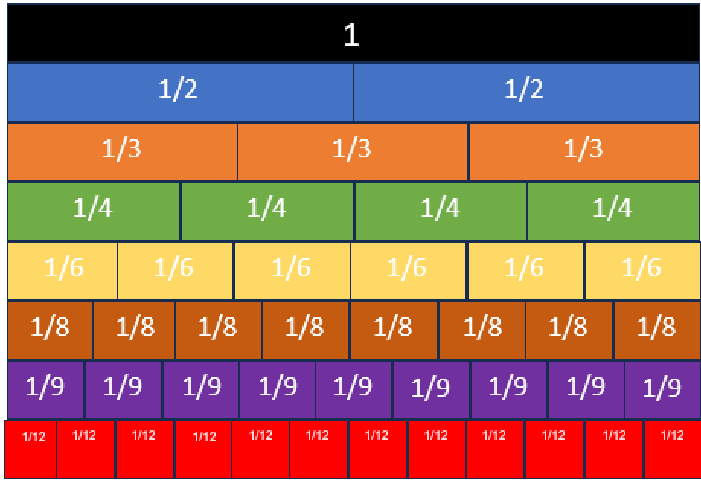
\includegraphics[width=0.6\linewidth]{Trabajos/06/Anexos/grafico_01}
		\caption{Fuente: elaboración propia}
		\label{fig:grafico_06_01}
	\end{figure}
	
	\item \textbf{Preguntas de reflexión durante la actividad:} \textit{¿Es posible plegar una tira de papel en 5 partes iguales? ¿Y en 7 partes iguales?} Estos interrogantes se plantean como propuestas de investigación para explorar más a fondo en sesiones posteriores, siguiendo el enfoque de investigación propuesto por Douady en el Juego de Marcos, que promueve la exploración y la experimentación como parte integral del aprendizaje matemático, por lo que se espera que los participantes a partir de esta experiencia, deduzcan la necesidad de un cambio de marco para dicha construcción, el geométrico.
	
	\item \textbf{Actividad grupal:} Una vez construido el Muro de Fracciones, los participantes se dividirán en \textbf{grupos} para reflexionar sobre la elaboración del material y las relaciones que emergen de él, tanto en términos de la totalidad como de las partes que lo componen, profundizando así en el significado de la fracción desde la perspectiva de las representaciones semióticas, analizando como diferentes representaciones pueden facilitar una comprensión más profunda del concepto de fracción.
	
	\item \textbf{Análisis comparativo:} También se les invita a analizar qué propiedades de los números naturales son aplicables y cuáles requieren ajustes en el contexto de las fracciones, apoyándose en las teorías de Duval y Duady para entender cómo las representaciones y marcos mentales influyen en la comprensión matemática.
	
	\item \textbf{Cierre:} Al concluir este primer encuentro sincrónico, se compartirá un Power Point con las ideas principales de las teorías de Duval y Doaudy que refuercen las lecturas sugeridas en la actividad previa.
	
	Utilizando el material creado, se les propondrá a los participantes crear un nuevo ``Muro de Fracciones'' que incluya las \textbf{fracciones equivalentes} encontradas durante la actividad, fomentando la aplicación práctica de los conceptos explorados.
\end{enumerate}

\subsubsection{Primeras tres horas entre clases}

\begin{enumerate}
	\item Se les solicitará que entreguen en la plataforma la resolución de la actividad:
	
	\begin{quote}
		\textit{Analicen y documenten utilizando el material Muro de Fracciones 3 formas diferentes de representar y obtener el entero. ¿Cómo estas representaciones pueden ser interpretadas por sus estudiantes? (primario-secundario)} Se sugiere subir un archivo Word en el que inserten imágenes de los muros que proponen con sus respectivas aclaraciones.
	\end{quote}
	
	\item Preguntas reflexivas: “\textit{¿Qué dudas u obstáculos podrían surgir entre sus estudiantes al realizar actividades con el muro de fracciones? ¿Cómo podrían abordarse estas dudas desde las teorías de Duval y Doaudy?}”
	
	\item Se compartirá un documento colaborativo en formato Drive, en el que los participantes harán breves intervenciones escritas destacando los hallazgos y análisis realizados. En él deberán considerar cómo estos podrían influir en su práctica docente y en la comprensión de sus estudiantes. De esta manera, se busca consolidar el aprendizaje desde los fundamentos teóricos y prácticos proporcionados por los organizadores del taller.
\end{enumerate}

\subsubsection{Segundas hora y media sincrónicas}

\begin{enumerate}
	\item Utilizaremos una presentación de Power Point para retroalimentar la corrección de la actividad entregada en el campus destacando cómo se puede validar la solución del plegado en 5 y 7 partes, a partir de los conceptos y métodos discutidos en el primer encuentro sincrónico.
	\item Continuaremos con la presentación para introducir el concepto de fracción como razón y su aplicación en la ubicación de números fraccionarios en la recta numérica utilizando el plegado de papel para ilustrar el concepto de manera visual y tangible.
	\item Procederemos a dividir a los talleristas en grupos y les asignaremos a cada grupo una actividad diferente, ordenarán fracciones en la recta utilizando como recurso el plegado de papel, un recurso privilegiado que colabora para que el alumno trabaje utilizando dicho sentido y no se presenten los obstáculos cognitivos de la representación en la recta utilizando procedimientos aritméticos.
	
	Se les propondrá entonces la resolución de actividades extraídas de:
	\begin{itemize}
		\item Itzcovich, Horacio. El Abecé de La Matemática Escolar. Capítulo 5: El trabajo escolar en torno a las fracciones, página 150.
		\item Documento curricular: Matemática: Fracciones y Números Decimales. Apuntes para la enseñanza. 6to grado. (2005). Gobierno de la Ciudad de Buenos Aires. Secretaría de Educación, página 17.
		\item Documento curricular: Matemática: Fracciones y Números Decimales. Apuntes para la enseñanza. 5to grado. (2005). Gobierno de la Ciudad de Buenos Aires. Secretaría de Educación, páginas 25, 26 y 27.
	\end{itemize}
	
	Luego, les propondremos reflexionar sobre las siguientes cuestiones:
	\begin{itemize}
		\itshape
		\item “¿Cuáles son los argumentos que un alumno, al finalizar 6to/7mo grado y de 1er año de secundaria estaría en condiciones de elaborar cuando resuelve este tipo de problemas?”,
		\item “¿Cómo crees que podría beneficiar en tus prácticas esta metodología de trabajo?”,
		\item “¿Qué fortalezas y debilidades puedes identificar en las resoluciones utilizando el plegado de papel?”
	\end{itemize}
	
	\item Cierre: Finalizado el momento de socialización de las diferentes resoluciones retomaremos las preguntas de reflexión para cerrar la actividad, animando a los participantes a implementar estas estrategias en sus prácticas.
\end{enumerate}

\subsubsection{Segundas tres horas entre clases}

\begin{enumerate}
	\item Deberán entregar en la plataforma en un archivo de Word actividades en las cuales deberán \textbf{ubicar números fraccionarios y decimales en la recta numérica a partir del uso del plegado de papel}.
	
	Las actividades serán extraídas de:
	\begin{itemize}
		\item Documento curricular: Matemática: Fracciones y Números Decimales. Apuntes para la enseñanza. 5to grado. (2005). Gobierno de la Ciudad de Buenos Aires. Secretaría de Educación, páginas 25, 26 y 27.
		\item Seoane, Silvana. Matemática material para docentes sexto grado educación primaria 1a ed. - Ciudad Autónoma de Buenos Aires: Instituto Internacional de Planeamiento de la educación IIPE-Unesco, 2012, páginas: 33 y 43.
	\end{itemize}
	
	\item El juego del \textbf{Tangram} favorece el pensamiento matemático, es un antiguo rompecabezas chino compuesto por 7 piezas: un cuadrado, un paralelogramo romboide y 5 triángulos semejantes diferentes. Los alumnos deberán ingresar al siguiente link: \url{https://www.youtube.com/watch?v=7wWQWUWHr5U} para construir el Tangram a partir del plegado de papel, este rompecabezas será el insumo para el Tercer encuentro sincrónico.
\end{enumerate}

\subsubsection{Terceras hora y media sincrónicas}

\begin{enumerate}
	\item Daremos comienzo a este último encuentro sincrónico con una presentación de Power Point para retroalimentar la actividad entregada en la segunda hora entre clases.
	\item Continuaremos con la presentación para reconstruir el recorrido realizado en los distintos momentos del taller: encuentros sincrónicos y momentos de estudio y de resolución de actividades asincrónicas, destacando los conceptos y sentidos de las fracciones, cómo llevarlos a la práctica con el uso de material tangible y los aportes de las teorías en los que se apoya este taller.
	\item Dividiremos a los talleristas nuevamente en grupos y les propondremos trabajar con una última actividad para poder relacionar y recuperar todo lo visto y analizado hasta el momento: El Tangram.
	\item Los invitaremos a reflexionar sobre:
	\begin{itemize}
		\item cómo surge el sentido de la fracción Parte-Todo y Parte de una parte,
		\item cómo hallar la medida de cada pieza del Tangram,
		\item las diferentes formas de hallar una parte del Tangram a partir de otras partes del mismo,
		\item equivalencias de áreas de diferentes figuras,
		\item cómo reconstruir figuras más pequeñas con las partes del Tangram, cómo hallar el área de la misma y su validación,
		\item relaciones de orden,
		\item los contenidos que circulan en las actividades,
		\item los conocimientos previos de los alumnos.
	\end{itemize}
	\item Finalizado el momento de trabajo grupal intervendremos para proponer la socialización sobre el análisis y reflexión de la propuesta de trabajo con el Tangram, destacaremos cómo puede invitarnos a repensar nuestras prácticas o futuras prácticas el uso de material didáctico al momento de abordar la enseñanza de las fracciones en el nivel primario y ciclo básico del secundario para favorecer el aprendizaje significativo de los estudiantes.
	\item Cerraremos el taller con unas palabras de reflexión a modo de conclusión. También, se les explicará que para acreditar el taller deberán completar una instancia evaluativa disponible en la plataforma.
\end{enumerate}

\subsubsection{Evaluación final}

\begin{enumerate}
	\item Para evaluar nuestra propuesta de taller, dejaremos disponible en la plataforma una encuesta que permitirá a los participantes realizar su feedback sobre la experiencia.
	\item Además, solicitaremos la entrega de la siguiente actividad para acreditar su participación en el Taller: "Redefiniendo el Sentido de las Fracciones: Aportes para su Enseñanza desde la Teoría de Representaciones Semióticas y el Juego de Marcos".
\end{enumerate}

\bigskip
\begin{center}
	\begin{minipage}{0.8\linewidth}
		\textbf{Actividad evaluativa}
		
		Buscar en libros de texto escolares del segundo ciclo de Educación Primaria y/o Ciclo Básico de la Escuela Secundaria una actividad que permita abordar la enseñanza de las fracciones en el sentido de Parte-Todo o como una Razón. Luego, analizar la misma a partir de preguntas que los inviten
		a reflexionar:
		\begin{itemize}
			\item ¿Qué conocimientos previos y habilidades matemáticas deben poner en juego los alumnos? Explica cómo la actividad puede ayudar a desarrollar una comprensión significativa de fracciones.
			\item Diversidad de representaciones: La actividad elegida, ¿propone la utilización de diferentes marcos y representaciones en su resolución? Identifique y describa brevemente.
			\item Integración de estrategias didácticas: ¿Que modificaciones sugerirías, para incorporar las estrategias de enseñanza de las fracciones con material didáctico vistas durante el taller? Describa cómo estos cambios podrían mejorar la comprensión de los estudiantes.
			\item Impacto en la práctica docente: ¿Cómo crees que las sugerencias propuestas podrían enriquecer tus prácticas docentes? Reflexiona sobre los posibles beneficios y desafíos de implementar estos cambios. ¿Qué conocimientos ponen en juego los alumnos al resolver dicha actividad?
		\end{itemize}
	\end{minipage}
\end{center}
\bigskip

Los participantes entregarán en un archivo Word la actividad elegida y su análisis. En la plataforma se habilitará un espacio creado para tal fin. Tendrán un plazo máximo de una semana (sujeto a revisión) para completar y subir el archivo de manera individual o en pareja. La corrección y devolución de las evaluaciones tendrán lugar por medio de la plataforma, con un plazo máximo de una semana (tiempo sujeto a revisión por parte de la organización).

\subsection{Bibliografía}

\nocite{*}
\printbibliography[keyword={06}]